\subsubsection{Syntax Trees}

Now that the parser for the given file has been generated by gt it is ready to be used. 
Figure 2.2 shows the syntax tree that is generated by the above grammar. Again, gt
can dump the Graph-viz file, but without Graph-viz installed it is not possible to see
the visual representation of a syntax tree or export them to images.
%
%
\begin{figure}[h!]
  \centering
  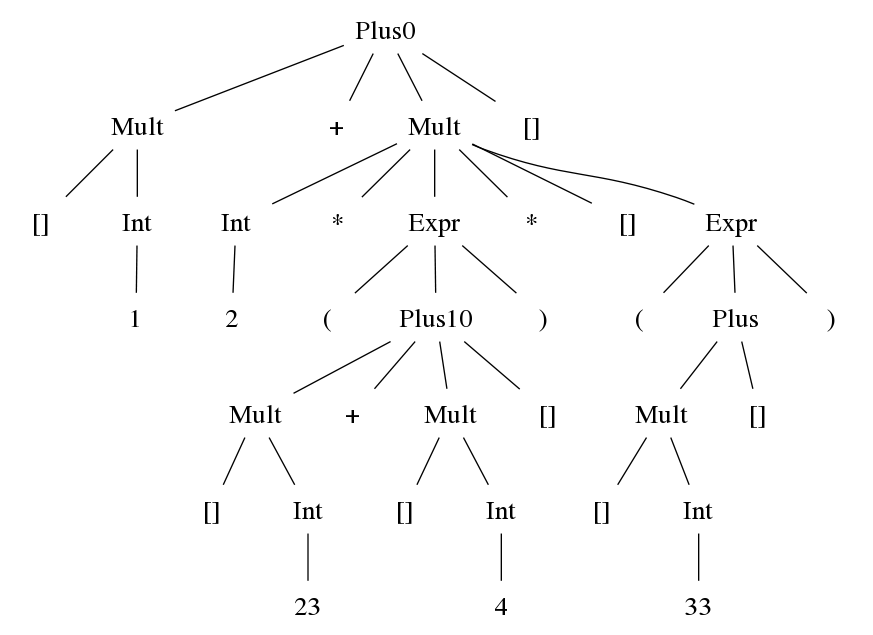
\includegraphics[width=4in]{./examples/ebnf/simple/ebnf-simple.png}
  \caption{Syntax Tree for\\ \textit{1 + 2 * (23 + 4) * (33)}}
\end{figure}







